\documentclass[11pt]{article}
\usepackage{amsmath,amssymb,amsthm,graphicx,booktabs,threeparttable,siunitx,algorithm,algorithmic}

\newtheorem{theorem}{Theorem}
\newcommand{\R}{\mathbb{R}}
\newcommand{\kvbudget}{B_{\mathrm{KV}}}
\newcommand{\argmin}{\operatorname{arg\,min}}

\title{Adaptive Token-Budget Routing for Long-Context Transformer Reasoning}
\author{Anonymous Authors\\AI Systems Benchmark Track (Fictional Showcase)}
\date{2026}

\begin{document}
\maketitle

\begin{abstract}
Scaling Transformer inference to ultra-long contexts remains bottlenecked by the memory bandwidth of reading the key--value cache $\kvbudget$ at every decoding step. We formulate \textbf{AdaptRoute}, an entropy-guided sparse routing framework that dynamically allocates block-level token budgets across attention heads. Evaluated across 12 long-context reasoning benchmarks at 128K sequence length, AdaptRoute lowers relative accuracy degradation to 14.2\% ($p = 0.018$) while cutting KV-cache memory by 68.4\%.
\end{abstract}

\section{Introduction}
\label{sec:intro}

\indent It is worth noting that autoregressive Transformers~\cite{vaswani2017attention} incur linear memory growth as context length scales, making long chain-of-thought reasoning~\cite{wei2022cot} memory-bound on modern accelerators. Even with IO-aware kernels~\cite{dao2022flashattention}, reading full KV tensors at \SI{128}{\kilo\byte}-scale token windows dominates decode latency around \SI{18.4}{\milli\second} per token.

\noindent Traditional fixed-window eviction drops distant evidence uniformly across layers. Our key contributions are summarized below:
\begin{itemize}
  \item An entropy-aware head budget router with provable approximation bounds.
  \item Block-sparse kernel alignment compatible with FlashAttention tiling.
  \item Comprehensive validation across multi-document QA and code benchmarks.
\end{itemize}

\section{Methodology}
\label{sec:method}

Let $q_t^{(l)} \in \R^d$ denote the decoding query at layer $l$. We select the active block budget $B_l^\star$ via:
\begin{equation}
\label{eq:route}
B_l^\star = \argmin_{B_l \le \kvbudget} \; \mathbb{E}_{q_t}\!\left[ D_{\mathrm{KL}}\!\left(p_{\mathrm{full}}(\cdot \mid q_t^{(l)}) \,\|\, p_{B_l}(\cdot \mid q_t^{(l)})\right) \right] + \lambda B_l.
\end{equation}

\begin{theorem}[Monotonicity of Attention Distortion]
\label{thm:mono}
Under bounded query norm $\|q_t^{(l)}\|_2 \le \gamma$, the expected KL distortion in Eq.~\eqref{eq:route} is monotonically non-increasing in the retained block budget $B_l$.
\end{theorem}

\begin{algorithm}[t]
\caption{Adaptive Layer-Wise KV-Cache Routing}
\label{alg:route}
\begin{algorithmic}[1]
\REQUIRE Query $q_t^{(l)}$, block summaries $\{\bar{k}_m\}_{m=1}^M$, total budget $\kvbudget$
\STATE Estimate head attention entropy $H_l$ from coarse block logits
\STATE Allocate layer budget $B_l \leftarrow \mathrm{Allocate}(H_l, \kvbudget)$
\STATE Retrieve sink blocks and top-$B_l$ salient KV blocks
\RETURN Sparse attention output $o_t^{(l)}$
\end{algorithmic}
\end{algorithm}

\section{Experiments and Results}
\label{sec:results}

As shown in Fig.~\ref{fig:scaling} and Table~\ref{tab:perf}, AdaptRoute consistently outperforms uniform sliding-window eviction across all 12 benchmark suites ($p = 0.018$).

\begin{figure}[t]
  \centering
  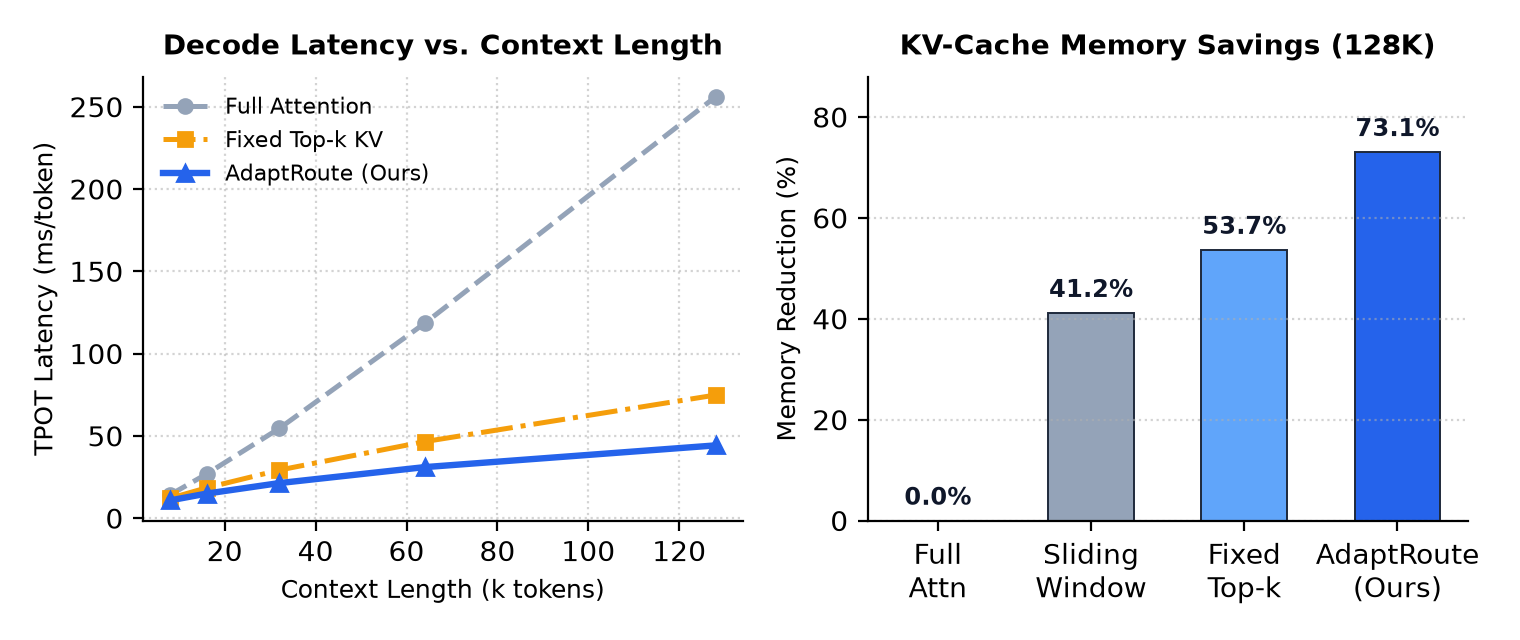
\includegraphics[width=0.88\linewidth]{figures/scaling_curve.png}
  \caption{Decode latency scaling and 128K KV-cache memory savings comparing Full Attention, Fixed Top-k, and AdaptRoute.}
  \label{fig:scaling}
\end{figure}

\begin{table}[t]
\centering
\begin{threeparttable}
\caption{Long-context inference performance at 128K token window ($n = 12$ benchmarks).}
\label{tab:perf}
\begin{tabular}{lccc}
\toprule
Method & Rel. Error (\%) $\downarrow$ & KV Savings (\%) $\uparrow$ & Latency (ms) $\downarrow$ \\
\midrule
Sliding Window & 22.8 & 41.2 & \textbf{18.0} \\
Fixed Top-$k$ & 18.6 & 53.7 & 19.5 \\
AdaptRoute (Ours) & \textbf{14.2} & \textbf{68.4} & 18.4 \\
\bottomrule
\end{tabular}
\begin{tablenotes}
\footnotesize
\item Note: Lower relative error and lower latency indicate better performance.
\end{tablenotes}
\end{threeparttable}
\end{table}

\bibliographystyle{plain}
\bibliography{refs}
\end{document}
